\chapter{Local Time Variation in Large-Scale Structure of Saturn's Magnetosphere}
\label{chap:LTsectors}
Throughout this thesis, we have shown how the large-scale structure of Saturn's magnetosphere is determined by internal and external factors, including the rapid planetary rotation rate, significant internal hot and cold plasma sources, and varying solar wind pressure. However it is still not fully understood which factors dominantly influence the configuration of the magnetosphere, and in particular how this relationship varies with local time. In this chapter, we explore this in detail using the UCL/AGA model Saturn's magnetodisc to describe the magnetosphere at different local time sectors. For model inputs, we use recent observational results which suggest a significant local time asymmetry in the pressure of the hot plasma population, and magnetopause location. We make calculations under different solar wind conditions, in order to investigate how these local time asymmetries influence magnetospheric structure for different system sizes. We find significant day-night asymmetries in the model magnetic field, consistent with recent empirical studies based on \textit{Cassini} magnetometer observations. We also find dawn-dusk asymmetries in equatorial current sheet thickness, with the varying hot plasma content and magnetodisc radius having comparable influence on overall structure, depending on external conditions. We also find significant variations in magnetic mapping between the ionosphere and equatorial disc, and ring current intensity, with substantial enhancements in the night and dusk sectors. These results have consequences for interpreting many magnetospheric phenomena that vary with local time, such as reconnection events and auroral observations. \\
\\
The content of this chapter is based on the study: \\
\\
\bibentry{sorba2019}. 

\section{Introduction to this Study}\label{LTsectors:sec:intro}
In recent years, a more global understanding of Saturn's magnetosphere has become possible largely thanks to the extensive temporal, spatial and seasonal coverage of the \textit{Cassini} space mission. \textit{Cassini} toured the Saturnian magnetosphere from 2004 to 2017, as described in detail in Chapter~\ref{chap:cassini}. In particular, there is now an opportunity to investigate in more detail how the large-scale structure of Saturn's magnetosphere varies with \textit{local time}, and which factors control this behaviour. This information is important for interpreting a range of phenomena at Saturn; for example the likelihood of reconnection events in different regions of the magnetosphere \citep{delamere2015}, which is related to how current sheet thickness varies with local time \citep{kellett2011}. Understanding more about the structure of the current sheet is also important for studies of the observed periodicities at Saturn's magnetosphere, which investigate the periodic modulation of the position and thickness of the equatorial current sheet, as in the study we presented in Chapter~\ref{chap:equinox}. More generally, a picture of the global magnetic field structure at different local times can be useful for understanding how different regions of the magnetosphere magnetically map to the polar ionosphere in different local time sectors, for example when interpreting observations of Saturn's aurora. The recently published empirical magnetic field model by \citet{carbary2018} suggests significant day-night asymmetry in equatorial-ionospheric magnetic mapping profiles, and local time asymmetries in the location of Saturn's aurora have been observed in studies such as \citet{badman2006,badman2011}.

A recent empirical study of magnetopause crossings by \citet{pilkington2015b} showed evidence of a dawn-dusk asymmetry in the typical location of the magnetopause boundary, with in general a larger magnetopause radius on the dawn flank. In addition, a survey of magnetospheric plasma populations from \citet{sergis2017} showed significant local time asymmetry in the hot plasma population, with enhanced pressures in the dusk and midnight local time sectors compared to dawn and noon. These factors will therefore influence the magnetic and plasma configuration of the magnetosphere differently at different local times. It was shown by \citet{achilleos2010b} that variations in the hot plasma pressure have a significant impact on the magnetospheric magnetic field configuration. They found that a globally elevated hot plasma pressure causes a more disc-like magnetic field structure, due to the enhancement of the equatorial ring current, and that this also influences the magnetic mapping between the equatorial disc and the ionosphere. We presented results consistent with this in Chapter~\ref{chap:compress}. We have also previously discussed in this thesis how our modelling results suggest that more expanded systems, with larger magnetopause radii, typically have a more disc-like magnetic field structure, due to overall force balance, and that this is consistent with other studies such as \citet{bunce2008} and \citet{arridge2008}. In particular \citet{arridge2008} found that in the noon sector, Saturn's magnetosphere only showed a significant divergence from a dipolar field structure for a magnetopause radius greater than ${\sim}\SI{23}{R_S}$, but that the magnetodisc structure is consistently observed on the dawn/dusk flanks and nightside.

In this work we investigate the relative importance of the hot plasma pressure and magnetopause radius asymmetries in controlling magnetospheric structure at different local time sectors using a modelling approach, to complement observational studies. We use the previously described UCL/AGA model, adapted to describe the typical, equilibrium conditions of Saturn's magnetosphere at four different local time sectors; noon (09:00-15:00), dawn (03:00-09:00), dusk (15:00-21:00) and night (21:00-03:00). We use equatorial profiles of the hot plasma pressure from \citet{sergis2017} for the different local time sectors as boundary condition inputs to the magnetodisc model, and determine appropriate magnetopause radius values to use for each sector based on the magnetopause surface model of \citet{pilkington2015b}. Our method of constructing these models is described in Section~\ref{LTsectors:sec:method}. In Section~\ref{LTsectors:sec:results} we present the results of these calculations, and highlight interesting comparisons in the magnetic field structure, azimuthal current density and magnetic mappings for the different local time sectors. Section~\ref{LTsectors:sec:conclusions} provides a brief summary of the main conclusions of this work.

\section{Method}\label{LTsectors:sec:method}
We use the UCL/AGA model first set out in \citet{achilleos2010a, achilleos2010b} and described in Section~\ref{intro:sec:forcebalancemodel}, with modifications to boundary conditions as described in Chapter~\ref{chap:equinox}, and additional modifications described in this section. As a reminder, this 2-D, axisymmetric force-balance model assumes the magnetospheric plasma comprises a cold population confined towards the rotational equatorial plane due to the centrifugal force exerted on it, and a hot population with associated plasma pressure $P_\mathrm{H}$ constant along magnetic field lines. The model calculates Saturn's magnetic field and plasma structure by iteratively solving a partial differential equation for the magnetic potential $\alpha$, and we consider the model to have converged when the relative difference between successive iterations falls below a given tolerance, as described in Section~\ref{intro:sec:forcebalancemodel}. In this study we found that, for nightside models with especially large disc radii, it was necessary to weight the previous solution up to nine times more heavily than the present solution in order to achieve convergence, corresponding to $\gamma=0.1$ in equation~(\ref{intro:eq:convergence}). This is a consequence of extending our use of this model to more extreme regimes.

As we have seen in this thesis, the UCL/AGA model was originally used to represent typical dayside conditions at Saturn, and so we made various modifications described herein, which are necessary to appropriately represent different local time sectors.

\subsection{Hot Plasma Parameterisation for Different Local Time Sectors}\label{LTsectors:sec:hotP}
\begin{table}
\caption[Coefficients of polynomial fits to the hot plasma pressure profiles from \citet{sergis2017}.]{Coefficients of fourth-order polynomial fits to the logarithm of each of the hot pressure profiles shown in Figure~\ref{LTsectors:fig:hotPpolys}, as described in the main text. } \label{LTsectors:tab:hotPpolys}
\centering
\begin{tabular}{c | c c c c}
%\hhline{-----}
\hline
Coefficient		& Noon						& Dawn			& Dusk				& Night	\\
%\hhline{-----}
\hline
$a_0$ 				&	-5.47						& -1.96 					&	-1.36					&	-6.86	 \\
$a_1$				&	1.10							& -0.149					&	-0.311					&	2.07	\\
$a_2$				&	-0.114						& 0.0686					&	0.109					&	-0.258 \\
$a_3$ 				&	0.00514					& -0.00652				&	-0.0104				&	0.0137 \\
$a_4$ 				&	\num{-8.47e-5} 		& \num{1.83e-4} 	&	\num{2.99e-4}	& \num{-2.71e-4}	\\
\hline
% \multicolumn{2}{l}{$^{a}$Footnote text here.}
\end{tabular}
\end{table}
\begin{figure}
\centering
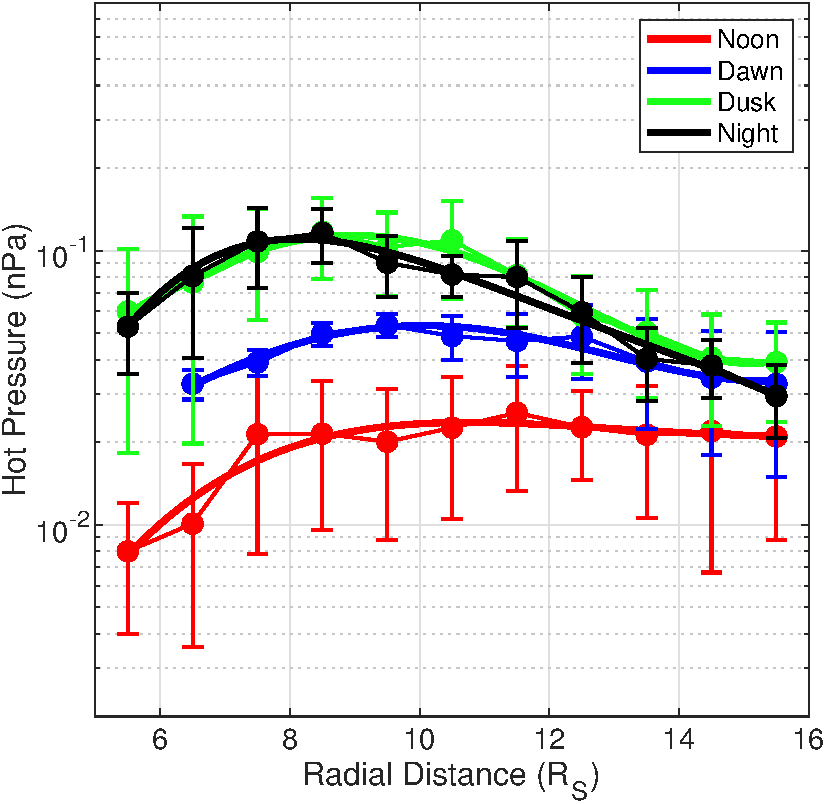
\includegraphics[width=0.6\textwidth]{LTsectors/hotPpolys.pdf}
\caption[Equatorial radial profiles of hot plasma pressure for different local time sectors from \citet{sergis2017}, with polynomial fits.]{Equatorial radial profiles of hot plasma pressure for different local time sectors, as shown by the colour. Solid circles and error bars are means and standard errors for binned data from \citet{sergis2017}, and solid lines are 4th order polynomial fits to the logarithms of the data points, as described in the main text.}
\label{LTsectors:fig:hotPpolys}
\end{figure}

The global hot plasma pressure is an important boundary condition for this model, as this strongly influences the resulting magnetic field structure. Recently, a comprehensive study using \textit{Cassini} MIMI data \citep{sergis2017} showed that the pressure of this hot plasma population not only varies over time and distance, but also varies significantly with local time, even when averaged over a large portion of the \textit{Cassini} mission (July 2004 - December 2013). Therefore in this study, we used average equatorial profiles of hot plasma pressure between $5.5$ and $\SI{15.5}{R_S}$ presented in \citet{sergis2017} for the different local time sectors, as boundary conditions for our models. Specifically, we fit the $\SI{1}{R_S}$-width-binned data presented in \citet{sergis2017} using polynomial functions of the form 
\begin{equation} \label{LTsectors:eq:fourthorderpoly}
\log(P_\mathrm{H}) = a_0+a_1\rho + a_2\rho^2 + a_3\rho^3 + a_4\rho^4
\end{equation}
following the approach used in \citet{sergis2017} for the total plasma population, with each point weighted by the inverse square of the provided standard error of the mean. The resulting coefficients for each sector are shown in Table~\ref{LTsectors:tab:hotPpolys}, with pressure in units of $\si{nPa}$ and radial distance in units of $\si{R_S}$. The best fit polynomials are shown in Figure~\ref{LTsectors:fig:hotPpolys}, as well as the corresponding observations from \citet{sergis2017}, with standard error of the mean of each bin shown by the error bars. This figure shows that the hot plasma pressure is significantly higher in the dusk and night sectors than the dawn and noon sectors. Here the dawn, noon, dusk and night sectors are defined by the magnetic local time intervals 03:00-09:00, 09:00-15:00, 15:00-21:00 and 21:00-03:00 respectively.

For values of $\rho$ smaller than the applicable range of the polynomials ($\SI{5.5}{R_S}$) we assumed the hot plasma pressure falls linearly to zero with $\rho$, broadly in line with observations and with the approach of \citet{achilleos2010a}. For the dawn profile we used an inner boundary of $\SI{6.5}{R_S}$ due to lack of data in the innermost bin in the \citet{sergis2017} data, which can be seen in Figure~\ref{LTsectors:fig:hotPpolys}. For values of $\rho$ above the applicable range of the polynomials ($\SI{15.5}{R_S}$), we assumed a profile where the product of the hot plasma pressure and the local flux tube volume is constant with radial distance, following previous studies such as \citet{achilleos2010a} and our study in Chapter~\ref{chap:compress}. In practice for the dawn and dusk models we used outer limits of $\SI{15.3}{R_S}$ and $\SI{15.1}{R_S}$ respectively, which are the locations of the local minima in the hot pressure polynomials, to ensure a smoother profile.

\subsection{Magnetopause Radius for Different Local Time Sectors}
\begin{table}
\caption[Details of the magnetodisc radius, shielding magnetic field value and $D_\mathrm{P}$ estimate for each local time sector model.]{Configuration details for the two families of models used to represent different local time sectors, for compressed (high solar wind dynamic pressure) and expanded (low solar wind dynamic pressure) regimes. magnetodisc radius, shielding magnetic field value and an estimate for the solar wind dynamic pressure $D_\mathrm{P}$ are shown for each model.}\label{LTsectors:tab:modelparams}
\centering
\begin{tabular}{l l c c c}
\hline
%Regime									&	LT Sector		& disc Radius ($\si{R_S}$)		& Shield $B_z$ ($\si{nT}$)		& $D_\mathrm{P}$ estimate ($\si{nPa}$)\\
Regime									&	LT Sector		& \makecell{Disc Radius \\ ($\si{R_S}$)}		& \makecell{Shield $B_z$ \\ ($\si{nT}$)}		& \makecell{$D_\mathrm{P}$ estimate \\ ($\si{nPa}$)}\\
\hline
\multirow{4}{*}{Compressed} & Noon			&	21.0										& -2.62									& \replaced{0.032}{0.031} \\
												& Dawn			& 34.3										& -0.97									& 0.026 \\
												&	Dusk			&	33.2										&	-0.88									& 0.030 \\
												& Night			& 42.0										& 0.14										&	- \\
\hline
\multirow{4}{*}{Expanded} 	& Noon			& 27.0										& -1.40									& 0.012 \\
												& Dawn			& 43.8										& -0.47									&	0.015 \\
												& Dusk				& 42.3										& -0.41									& 0.016 \\
												& Night			& 54.0										& 0.13										& - \\
\hline
\end{tabular}
\end{table}

The UCL/AGA model used can also be parameterised by an effective disc radius $R_\mathrm{D}$, the equatorial radial distance of the last closed field line in the model. As discussed in Section~\ref{LTsectors:sec:intro} and throughout this thesis, variations in this quantity also significantly impact the resulting magnetic field structure in the model. It was therefore important for this work that we chose appropriate values of the disc radius $R_\mathrm{D}$ for each of the local time sectors we were describing. To do this, we appealed to the study of \citet{pilkington2015b}, who improved the earlier Saturn magnetopause surface models of \citet{pilkington2015, kanani2010, arridge2006} by in particular including a small dawn-dusk asymmetry in magnetopause radius in the model. In \citet{pilkington2015b} the authors used observations of magnetopause crossings made throughout a large portion of the \textit{Cassini} mission to constrain parameters for a \citet{shue1997} type magnetopause model, introducing an extra parameter to describe the dawn-dusk asymmetry whilst maintaining a continuous surface at the magnetopause nose. They found that on average the magnetopause boundary extends farther from the planet on the dawn side than the dusk side, by ${\sim}7\%$. 

In order to investigate how local time variation in magnetospheric structure varies with system size, we calculated two sets of models under different solar wind dynamic pressure conditions; a compressed regime with subsolar magnetopause radius fixed at $\SI{21}{R_S}$, and an expanded regime with subsolar magnetopause radius fixed at $\SI{27}{R_S}$, following the bimodal values observed in \citet{pilkington2015} and \citet{achilleos2008}. For the corresponding dawn and dusk disc radii, we calculated the magnetopause radius at the centre of each local time sector (06:00 for dawn and 18:00 for dusk) using the best fit parameters given in \citet{pilkington2015} and \citet{pilkington2015b}. We used a value of the nose plasma $\beta = 3$, which is the median value for the dataset of magnetopause crossings provided in \citet{pilkington2015}, although for a fixed subsolar radius this choice of $\beta$ had very little impact on the resulting flank radii. Thus we determined the appropriate disc radii $R_\mathrm{D}$ for noon, dawn and dusk local time sectors, for both high and low solar wind pressure conditions. The resulting values are shown in Table~\ref{LTsectors:tab:modelparams}. In the absence of an accurate magnetopause model for the nightside of Saturn's magnetosphere, we used a disc radius of twice the subsolar magnetopause radius to represent an approximate nightside local time sector structure.

The solar wind dynamic pressure corresponding to a given equilibrium magnetodisc model can be estimated by assuming pressure balance across the boundary at the equator, as in Chapters~\ref{chap:compress} and \ref{chap:equinox}. Specifically we can assume
\begin{equation}\label{LTsectors:eq:pbalance}
\frac{B_\mathrm{MS}^2}{2\mu_0} + P_\mathrm{MS} = \left[k\cos^2(\psi) + \frac{k_\mathrm{B}T_\mathrm{SW}}{1.16m_\mathrm{p}u_\mathrm{SW}^2}\sin^2(\psi)\right] D_\mathrm{P} \tag{\ref{intro:eq:pbalance2} revisited}
\end{equation}
where terms on the left hand side represent the magnetospheric magnetic and plasma pressures just inside the magnetopause boundary, and the terms on the right represent the component of solar wind dynamic pressure incident on the magnetopause surface, and a smaller component associated with the solar wind's thermal pressure. As before, $k = 0.881$ is a factor to account for the diversion of flow around the magnetosphere obstacle \citep[see][]{spreiter1966}, $k_\mathrm{B}T_\mathrm{SW} = \SI{100}{eV}$ and $u_\mathrm{SW} = \SI{460}{\km\per\second}$ are the temperature and speed of the solar wind from \citet{pilkington2015}, and $\psi$ is the angle between the incident solar wind and the magnetopause surface normal. We used values for $B_\mathrm{MS}$ and $P_\mathrm{MS} = P_\mathrm{H} + P_\mathrm{C}$ extracted just inside the magnetopause boundary of each model, and obtained $\psi$ from the \citet{pilkington2015b} magnetopause surface model at the appropriate local time sector. The resulting estimates of $D_\mathrm{P}$ are shown in Table~\ref{LTsectors:tab:modelparams}. This approach is not appropriate for the far night-side tail, where a concept of $\psi$ is not directly applicable, and so we do not attempt to estimate $D_\mathrm{P}$ for those sector models. While the values of $D_\mathrm{P}$ do not exactly agree for all compressed or all expanded models, we can see that the two regimes provide significantly different, self-consistent estimates. The mean $D_\mathrm{P}$ estimates are $0.029\pm\SI{0.003}{nPa}$ and \replaced{$0.014\pm\SI{0.002}{nPa}$}{$0.015\pm\SI{0.002}{nPa}$} for the compressed and expanded regimes respectively, such that they broadly correspond systems under different solar wind conditions, whilst representing average internal conditions.

\subsection{Magnetodisc Model Adaptations}\label{LTsectors:sec:adaptations}
Finally, we made minor adaptations to the magnetodisc model construction in order to be more appropriate for different local time sectors. As discussed elsewhere in this thesis, in \citet{achilleos2010a} the authors include a small, uniform, southward-directed `shielding field' to the total magnetic field at every iteration, to approximately account for the magnetic field associated with the magnetopause and magnetotail current sheets. The magnitude of this field was chosen by calculating dayside equatorial averages of the empirical field models of \citet{alexeev2005} and \citet{alexeev2006}, and it varied with model magnetodisc radius $R_\mathrm{D}$. For this study, we calculated local time sector averages of these field models over circular segments with radius $R_\mathrm{D}$, to account for the increased significance of the tail current field compared to the magnetopause current field for nightside local time sectors in particular. We also enhanced the field associated with the magnetopause current beyond a dipole approximation by a factor $(1+k_\mathrm{MD})$, where $k_\mathrm{MD}$ is the ratio of the ring current and planetary dipole magnetic moments, as in the study in Chapter~\ref{chap:equinox}. As described in Section~\ref{equinox:sec:modmodifications}, to estimate the appropriate $k_\mathrm{MD}$ for each model we employed an extrapolation of the empirical linear fit from \citet{bunce2007}, although here we used our values of $R_\mathrm{D}$ rather than the subsolar magnetopause radius to estimate $k_\mathrm{MD}$ as we found that this in particular improved convergence in our models. The resulting values for the shielding magnetic field $B_z$ for each model are shown in Table~\ref{LTsectors:tab:modelparams}. It can be seen that, as expected, the total shielding field decreases and becomes northward directed for the nightside models due to the increased influence of the more northward field associated with the distant tail currents, compared to the more southward field associated with magnetopause currents. While the use of these shielding field values does not significantly affect the global magnetic field structure of the resulting models, we find it does improve the tendency for our models to achieve convergence.

We also updated the representation of the cold equatorial ion temperatures used as a boundary condition in the UCL/AGA model, using a recent comprehensive survey of equatorial \textit{Cassini} CAPS observations from \citet{wilson2017}. We fit the equatorial profiles of parallel and perpendicular temperatures for hydrogen and water group ions between $5.5$ and $\SI{30}{R_S}$ presented in \citet{wilson2017} with fourth-order polynomials, with points weighted by the inverse square of the error (assumed to be half the interquartile range of each bin). We then derived a single equatorial plasma temperature profile for the magnetodisc model as in \citet{achilleos2010b}, who used the same approach but with earlier more restricted data sets from \citet{wilson2008} and \citet{mcandrews2009}. The best fit polynomials for each ion species and temperature moment are given in the Appendix~\ref{appendix:sec:temperature}, along with a comparison of the original profiles from \citet{achilleos2010b}. We found that this modification did not significantly affect the overall resulting magnetic field profile of the magnetodisc model, in general causing only a slight increase in magnetic field strength in the inner magnetosphere, and slight decrease in the outer magnetosphere, with a maximum difference under $\SI{1}{nT}$. However this modification did improve model estimates of the cold plasma pressure, reducing the values in the outer magnetosphere such that they showed better agreement with recent observations from \citet{sergis2017} (also based on CAPS data). This modification represents better radial coverage and global constraint of the cold plasma temperature than in previous studies.

\section{Results and Discussion}\label{LTsectors:sec:results}
\subsection{Magnetic Field Structure}
The equatorial magnetic field profiles from the resulting magnetodisc models for each local time sector are shown in Figure~\ref{LTsectors:fig:eqBfield}. For comparison, a representative profile for the internal planetary dipole magnetic field is shown by the grey dashed line on each plot.

\begin{figure}
\centering
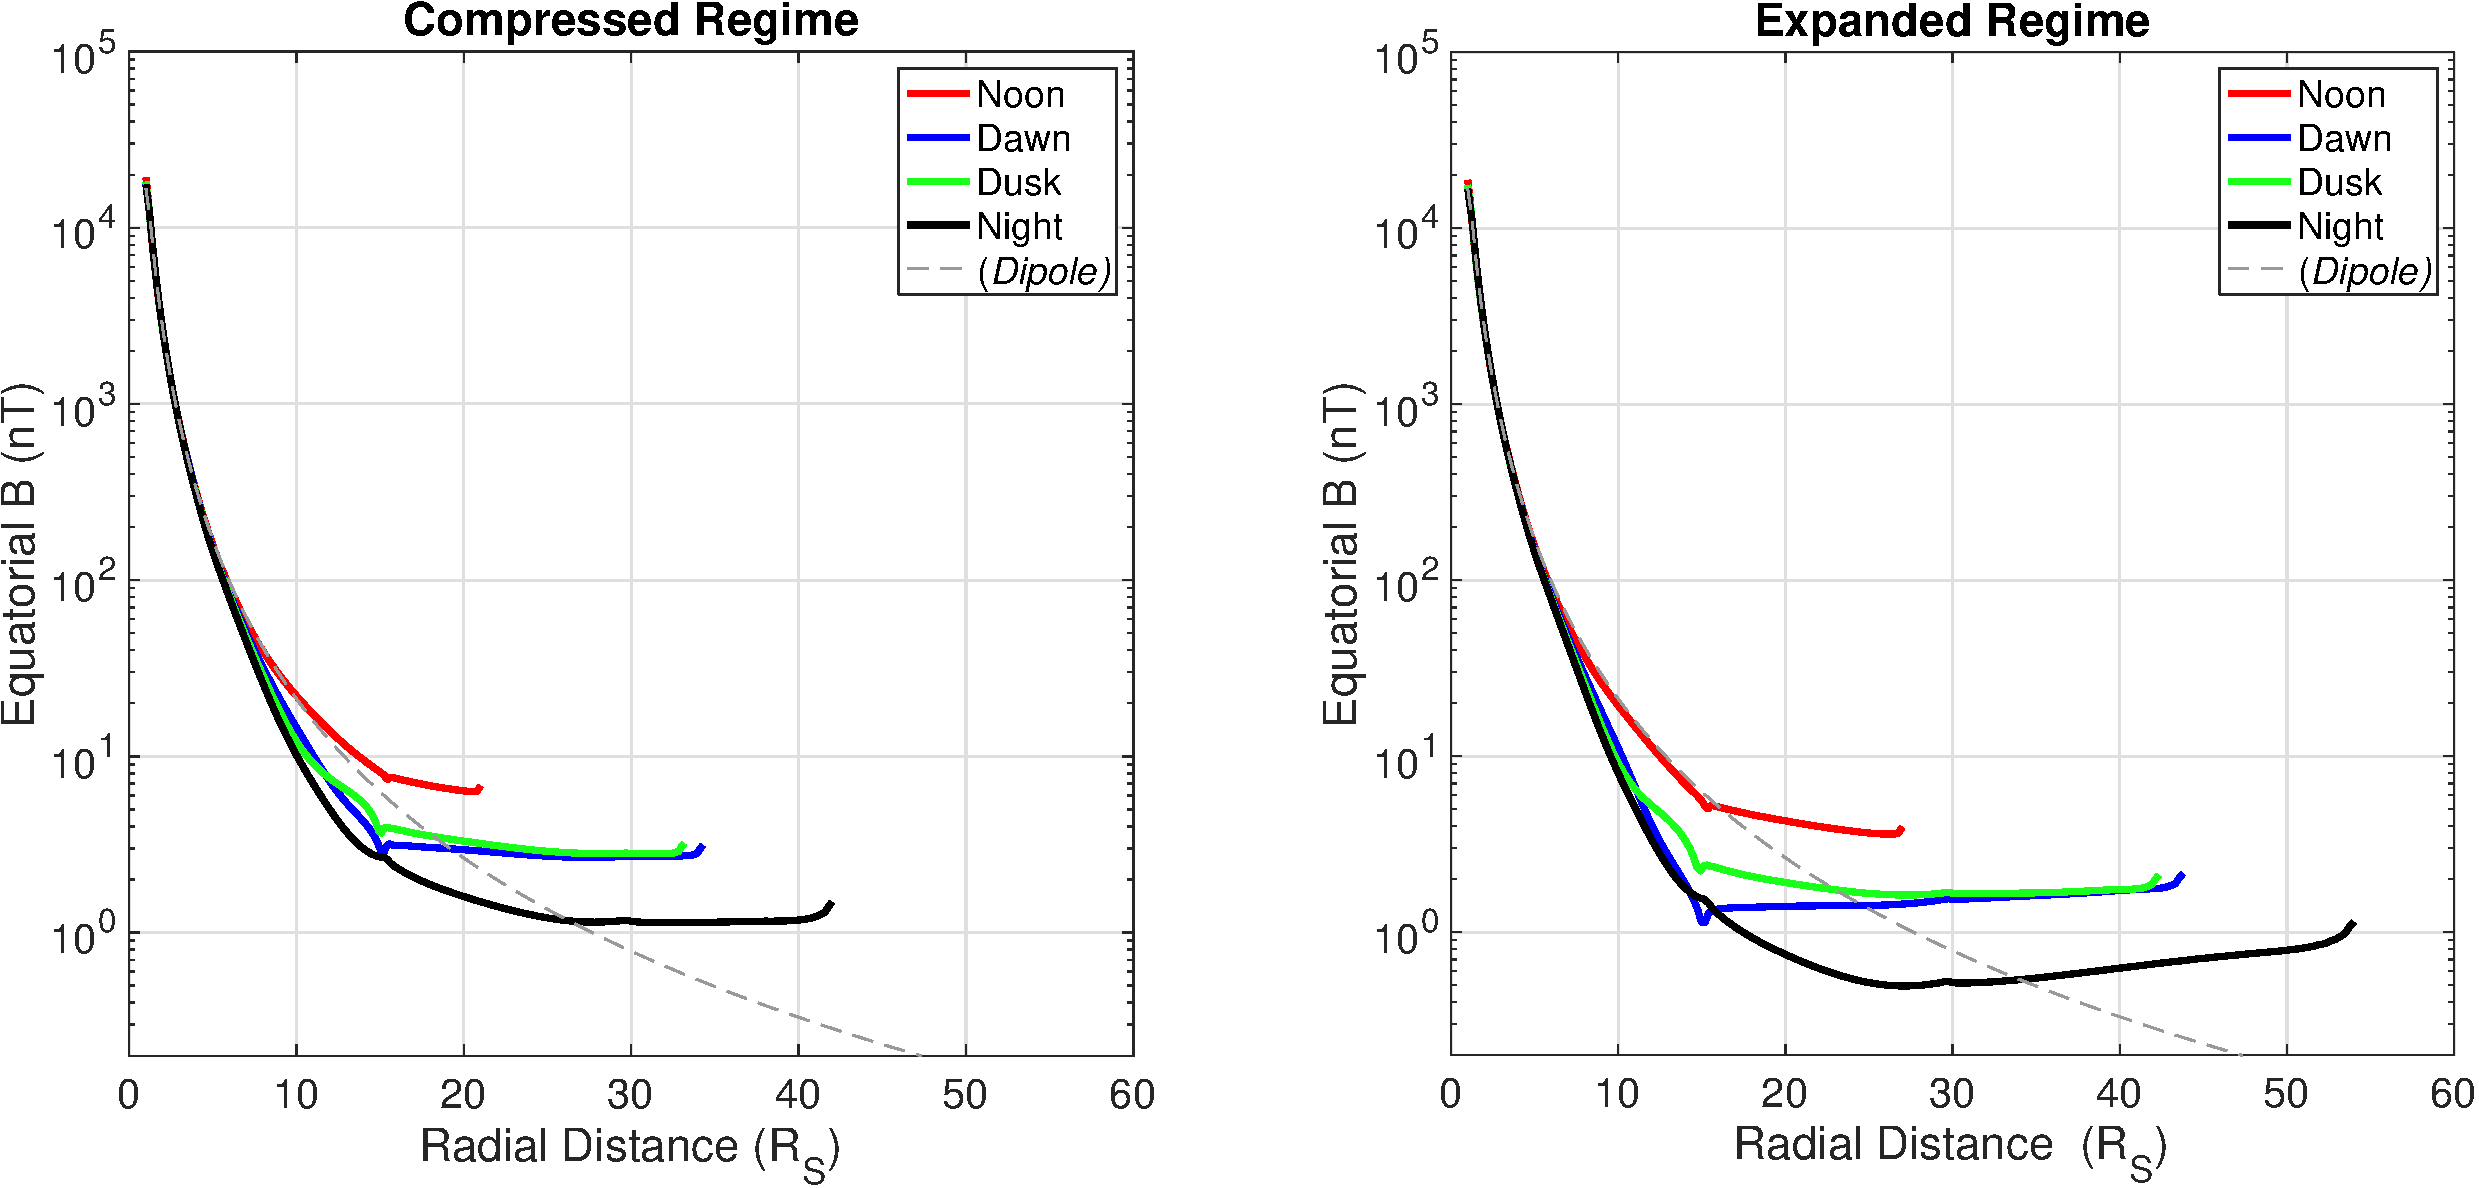
\includegraphics[width=0.8\textwidth]{LTsectors/eqBfield.pdf}
\caption[Model equatorial profiles of magnetic field strength $B$ for different local time sectors, for compressed and expanded regimes.]{Equatorial profiles of total magnetic field strength $B$ with radial distance for each local time sector as shown by the colour, for both the compressed (a) and expanded (b) regimes. On each plot a profile for a dipole magnetic field is shown in dashed grey for comparison.}
\label{LTsectors:fig:eqBfield}
\end{figure}

For the dayside (noon) models, we can see that the magnetic field is approximately dipolar in the inner ($\lesssim\SI{10}{R_S}$) magnetosphere, and falls more slowly with radial distance than a dipole in the middle ($10\lesssim\rho\lesssim\SI{15}{R_S}$) and outer magnetosphere. This behaviour broadly corresponds to a more disc-like magnetic field structure compared to a dipole, and appears for a more significant range in radial distance for the expanded noon model. This reconfiguration at larger system size is consistent with the aforementioned \textit{Cassini} observations from \citet{arridge2008}, and ring current modelling from \citet{bunce2008}.

For the larger dawn, dusk, and night sector models, the model magnetic field strengths are lower than the corresponding dipole field in the inner magnetosphere, and greater in the outer magnetosphere. This too is in line with \textit{in situ} observations of Saturn's magnetosphere, such as \citet{delamere2015}, who analysed equatorial current sheet crossings using \textit{Cassini} MAG data, in order to demonstrate how the equatorial magnetic field varies with radial distance in different local time sectors. There is also a small dawn-dusk asymmetry in the magnetic field strengths in our model, with the dusk sector profile persistently higher than the dawn in the middle and outer magnetosphere. This is likely a consequence of force balance, with the slightly higher hot plasma pressure in the dusk sector requiring a greater magnetic curvature force to balance it, provided by a greater magnetic field strength. This is interesting to note, as such a small asymmetry in field strength would be unlikely to reveal itself in observational studies of Saturn's magnetosphere, especially due to the relatively poor sampling of the dawn sector equatorial magnetosphere by the \textit{Cassini} spacecraft over its mission.

\begin{figure}
\centering
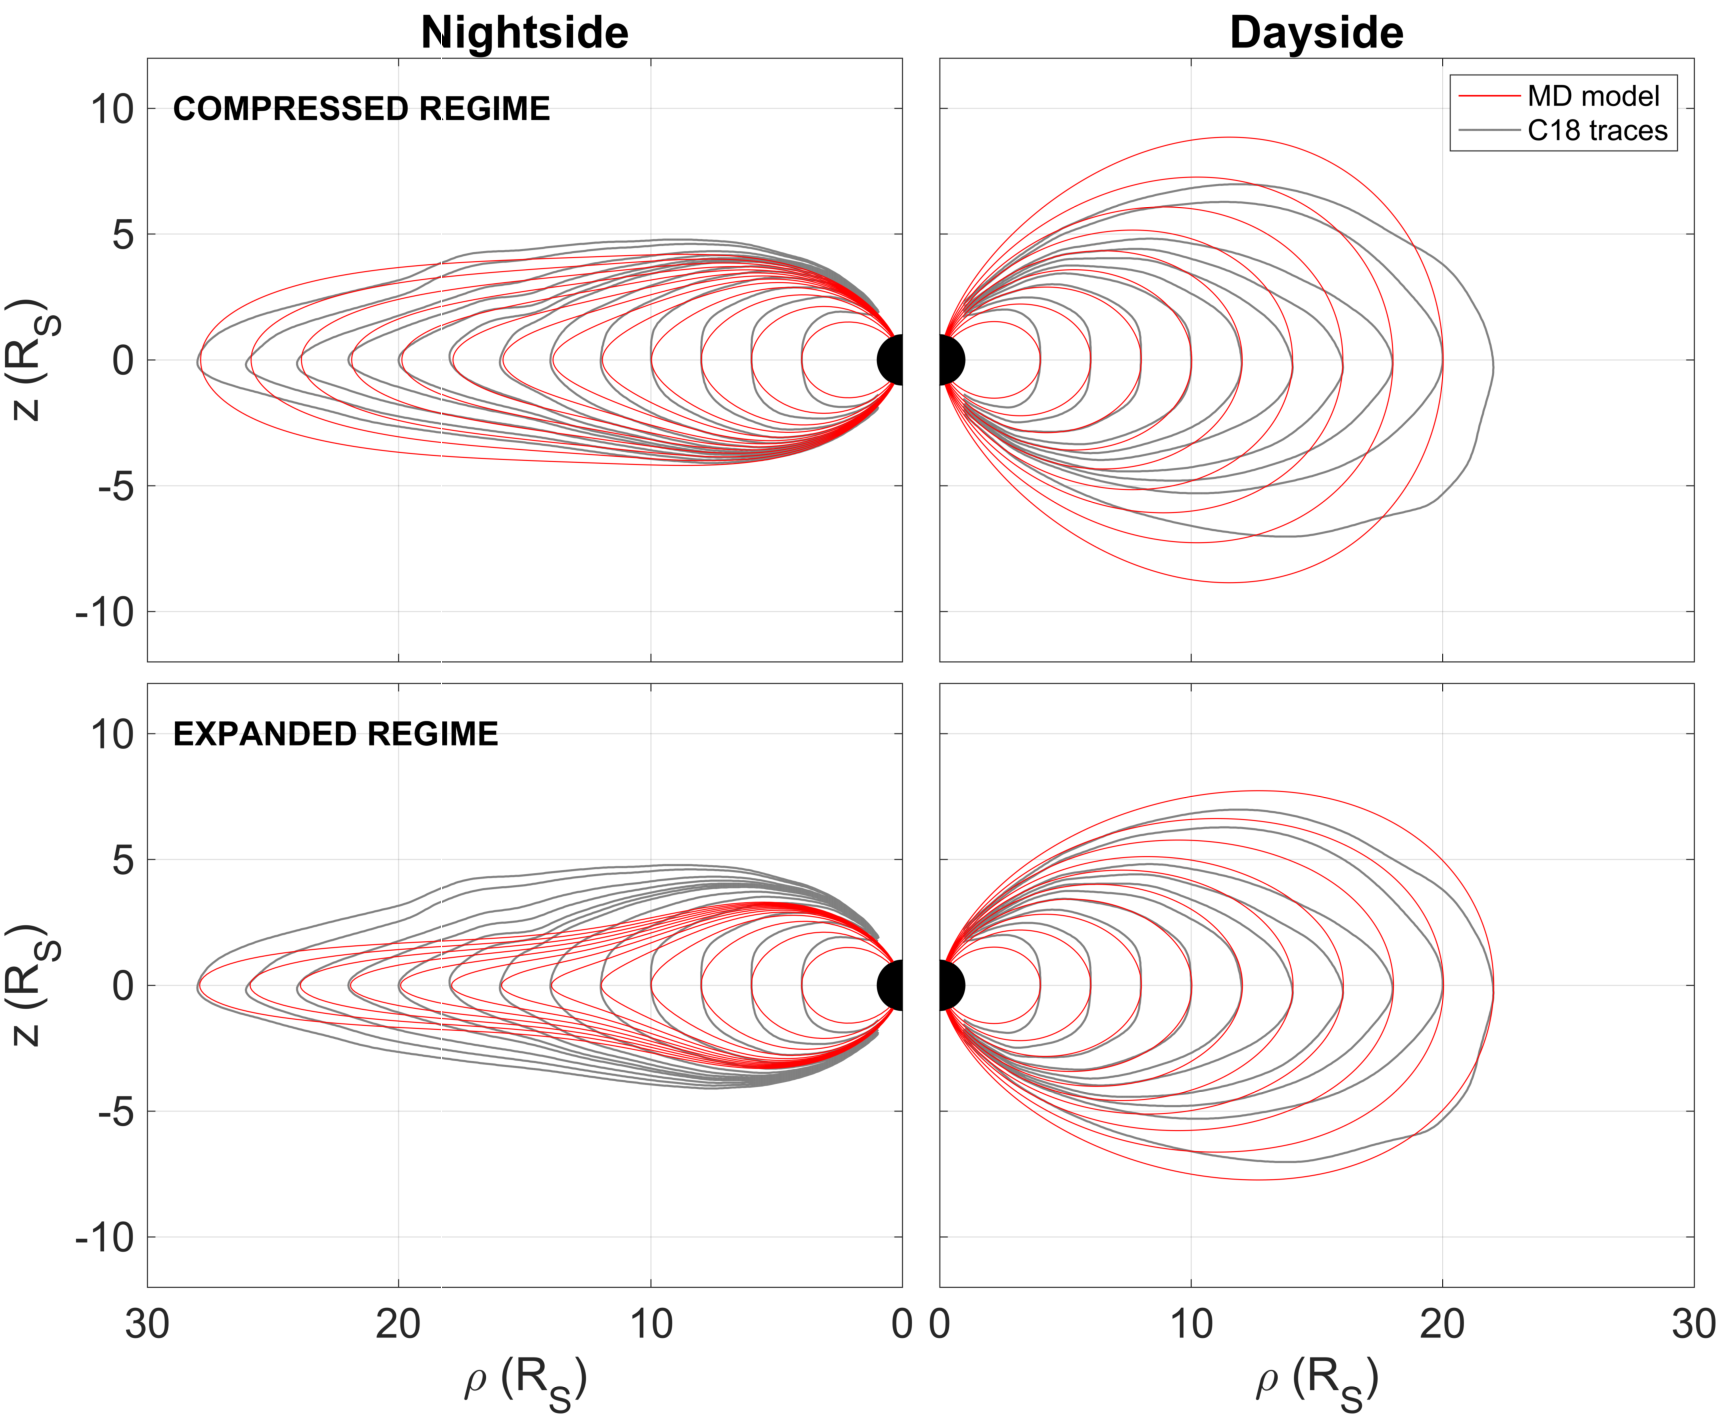
\includegraphics[width=0.7\textwidth]{LTsectors/carbarycomparison.pdf}
\caption[Model magnetic field lines for the dayside and nightside models, for the compressed and expanded regimes, compared to \citet{carbary2018} results.]{A comparison of model magnetic field lines from \citet{carbary2018} and this study. In grey are shown \replaced{traces based on}{polynomial fits to} binned \textit{Cassini} magnetometer meridional magnetic field observations from \citet{carbary2018} (top and bottom panels an exact reproduction). In red are shown magnetic field lines from the noon and nightside models presented in this study, for the compressed (top panel) and expanded (bottom panel) regimes, for L shells to match those of the \citet{carbary2018} study.}
\label{LTsectors:fig:carbarycomparison}
\end{figure}

Looking at the day-night asymmetry in more detail, in Figure~\ref{LTsectors:fig:carbarycomparison} we show the magnetic field structure for our noon and nightside magnetodisc models, for the compressed (top panel) and expanded (bottom panel) regimes\added{ in the range $\rho = 4{\--}\SI{22}{R_S}$ for the dayside and $\rho = 4{\--}\SI{28}{R_S}$ on the nightside, noting that our compressed dayside model only extends out to $\rho = \SI{21}{R_S}$}. For comparison, we include in \replaced{grey}{red} \replaced{field line traces based on empirical observations}{an empirical magnetic field model} from a recent study by \citet{carbary2018}. In that study the author binned magnetic field observations from almost the entire \textit{Cassini} mission into two local time sectors, dayside and nightside, and \replaced{calculated traces using a Runge-Kutta propagator \citep[see][and references therein for more details]{carbary2018}}{fit these using polynomial functions of latitude in order to derive a simple analytical model of Saturn's meridional magnetic field lines}. \citet{carbary2018} accounted for seasonal warping of the current sheet via a coordinate transformation\replaced{, however}{, although the polynomial functions still include terms that enable asymmetry across the rotational equator. However} unlike in this study, \deleted{the }\citet{carbary2018} did not account for a change in external solar wind conditions, and so we have reproduced the same \replaced{traces}{model output} from \citet{carbary2018} in the top and bottom panels. 

We can see that the overall magnetic field structures in our models are similar to those of the \citet{carbary2018} model, in particular the expanded $R_\mathrm{D} = \SI{27}{R_S}$ dayside model, and the compressed $R_\mathrm{D} = \SI{42}{R_S}$ nightside model. \deleted{In addition, the somewhat blunt, `blockish' shape of the dayside field lines in the \citet{carbary2018} model are somewhat accentuated by the polynomial representation the author used, with the original traces of field lines presented in that study showing a structure even more similar to our models presented here. }Only our expanded nightside model shows a magnetic field structure that is significantly more disc-like than the \citet{carbary2018} analytical model, suggesting that perhaps a magnetodisc radius of $\SI{54}{R_S}$ is somewhat too extreme to accurately characterise the typical midnight magnetosphere. However in general the agreement is good, suggesting our models can characterise the overall structure of the magnetospheric magnetic field at different local times, provided the model disc radius is chosen appropriately. Also, we should note that here we are comparing specifically our noon (LT \replaced{09:00-15:00}{03:00-09:00}) and night (LT 21:00-03:00) sector models with the \citet{carbary2018} \replaced{traces}{models} which correspond to wider, 12 hour local time regions. Therefore to more accurately represent (for example) the entire dayside for a more direct comparison, we would need to consider some combination of our noon, dawn and dusk sector model outputs.

\begin{figure}
\centering
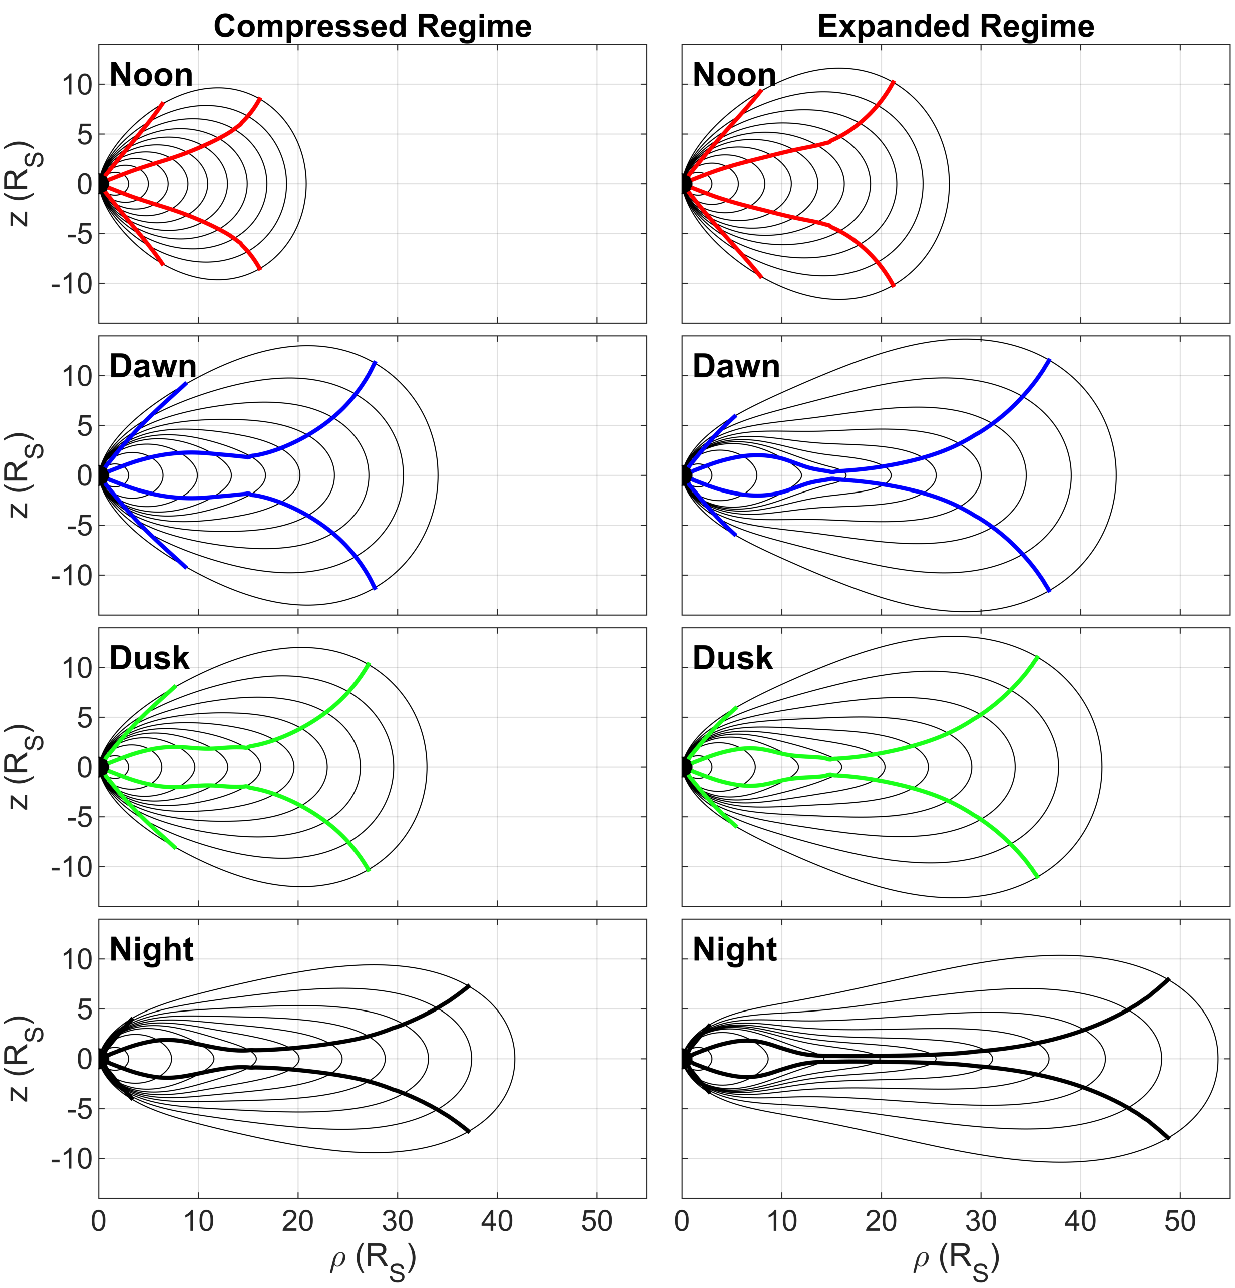
\includegraphics[width=0.8\textwidth]{LTsectors/discyness.pdf}
\caption[Model magnetic field structures for different local time sectors, with bounding lines showing regions where the magnetic field direction is within $\SI{30}{\degree}$ of the equatorial plane.]{The magnetic field structure for each magnetodisc model for the compressed (left column) and expanded (right column) regimes, shown by the solid black lines. Superposed in colour for each model are pairs of lines in each hemisphere which bound regions where the local magnetic field direction lies within $\SI{30}{\degree}$ of the equatorial plane.}
\label{LTsectors:fig:discyness}
\end{figure}

\begin{figure}
\centering
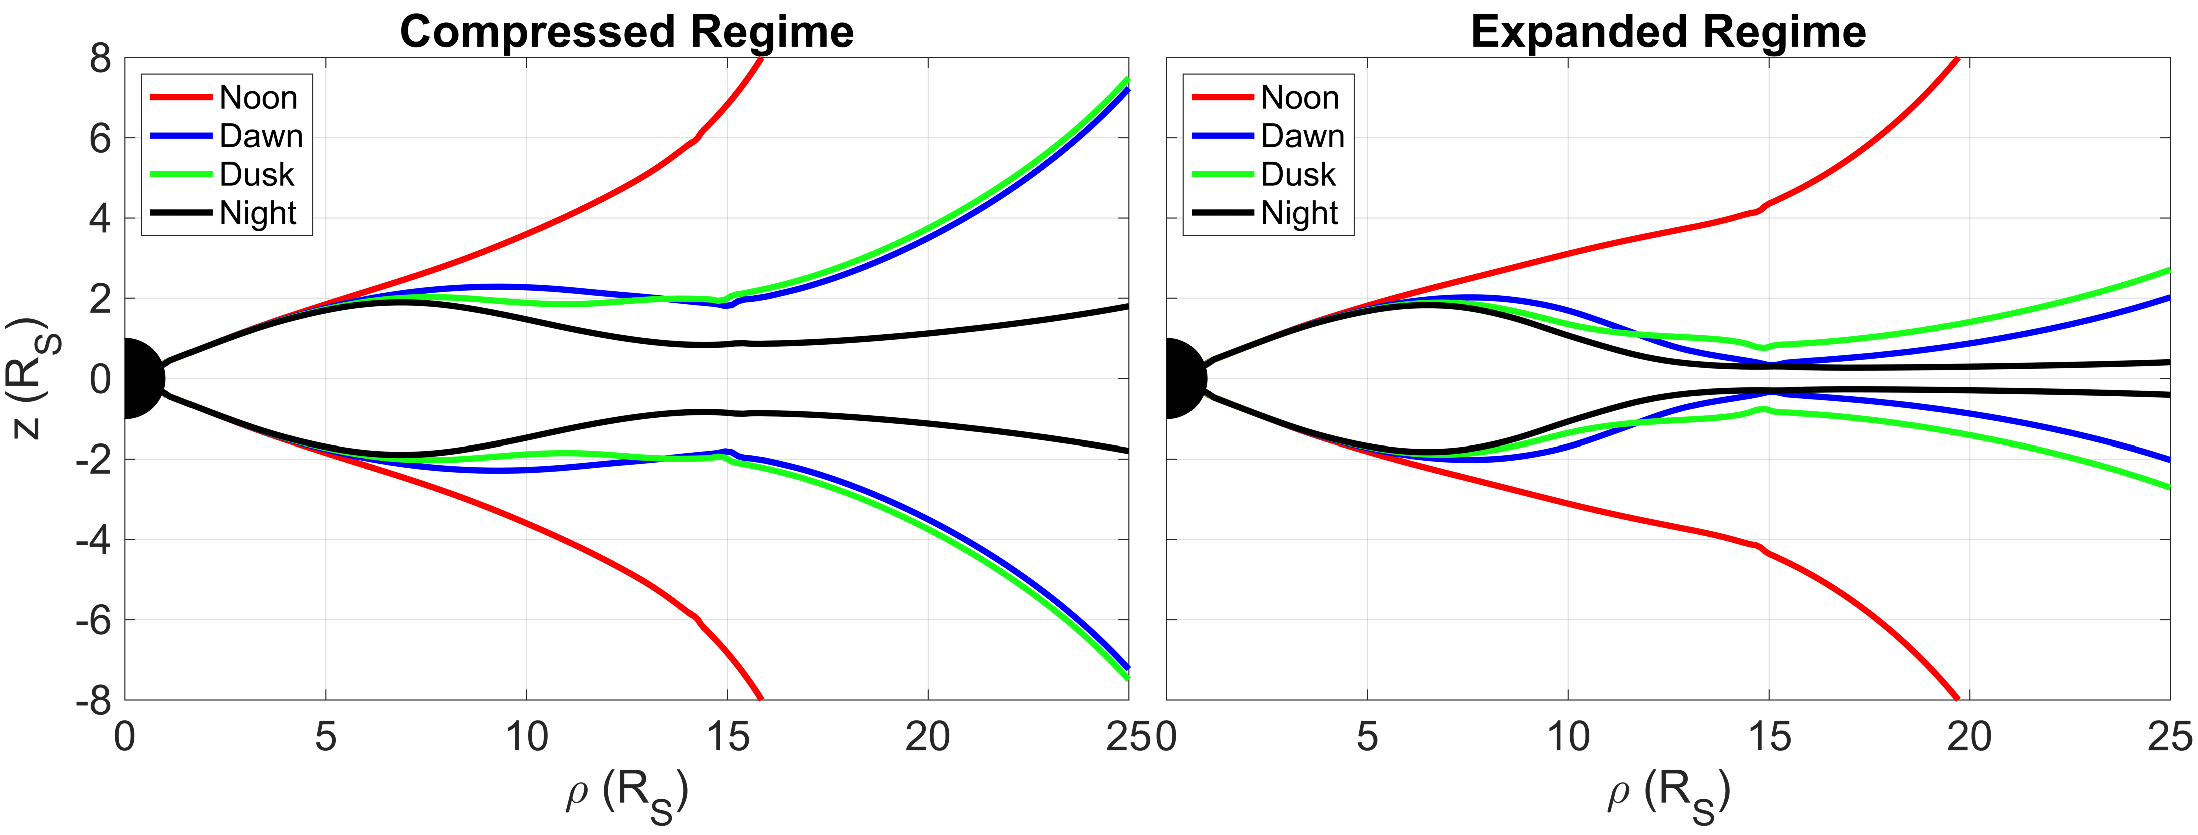
\includegraphics[width=0.8\textwidth]{LTsectors/discyness2.pdf}
\caption[Reproduction of the lower latitude bounding lines from Figure~\ref{LTsectors:fig:discyness}.]{Reproduction of the more equatorward coloured lines from Figure~\ref{LTsectors:fig:discyness}, for each local time sector model, for compressed (left) and expanded (right) regimes. These represent the low latitude boundaries of regions where the local magnetic field direction lies within $\SI{30}{\degree}$ of the equatorial plane.}
\label{LTsectors:fig:discyness2}
\end{figure}

In order to investigate more just how `disc-like' the magnetic field is in each local time sector, we use a visualisation technique employed in \citet{bunce2008}, where for each model we bound regions of the magnetosphere where the local magnetic field direction lies within $\SI{30}{\degree}$ of the equatorial plane, such that the field lines are approximately parallel to the equatorial plane. The results are shown in Figure~\ref{LTsectors:fig:discyness}, and the reproduction of the most lower latitude of the bounding lines are shown in Figure~\ref{LTsectors:fig:discyness2}. The magnetic field structure for each model is also shown in black, to further illustrate how this method characterises the `discy-ness' of the magnetic field structures. These figures show that, as expected, the larger magnetodisc models have significantly more disc-like magnetic field structures in the middle magnetosphere, than the smaller, more dipolar models, as shown by bounding lines that are closer to the equator. As previously discussed, this was observed in previous studies such as \citet{achilleos2010a} and the study in Chapter~\ref{chap:compress}, and is a result of how the overall force-balance within the magnetosphere changes with system size, in terms of the dominant magnetic and plasma related forces. 

In addition, from Figure~\ref{LTsectors:fig:discyness2} in particular, it can be seen that, for the compressed regime, the dusk sector has a slightly thinner and more disc-like magnetodisc structure in the middle magnetosphere than the dawn sector, as shown by the bounding lines being more equatorward for the dusk model (shown in green). This effect is likely due to the local enhancement of the ring current in the dusk sector due to the increased hot plasma pressure, which causes a more extreme perturbation from a dipolar magnetic field. This was also observed in \citet{achilleos2010b} and the study in Chapter~\ref{chap:compress}. Note that this `thinning' of the disc is not the same as thinning of the \textit{plasma} sheet, which is made up of both hot and cold plasma populations. While the \textit{current} sheet and associated \textit{cold} plasma sheet thins, the hot plasma is actually more populous for the thinner, dusk model, and the associated hot plasma pressure is constant along magnetic field lines. As described in \citet{sergis2011} and \citet{arridge2009b} the current sheet, a predominantly magnetic structure, has been observed to be thinner than the plasma sheet it is embedded in, and the plasma sheet itself can have different thicknesses in different particle energies and species.

For the expanded regime, it can be seen in Figure~\ref{LTsectors:fig:discyness2} that the opposite relationship is true, and that in the middle and outer magnetosphere, the dawn sector magnetic field has a thinner and more disc-like structure (shown in \deleted{light }blue). This is likely due to the increased influence of the dawn-dusk asymmetry in effective magnetodisc radius for the expanded regime, as a larger magnetopause radius also promotes a more disc-like structure. For the expanded regime, the dawn magnetopause is $\SI{1.5}{R_S}$ greater than the dusk, compared to $\SI{1.1}{R_S}$ for the compressed regime. 

It is interesting that this transition in dominant behaviour occurs across this compressed-expanded regime threshold. These results suggest that the asymmetries in magnetopause radius and hot plasma content have comparable influence on the global magnetic field structure in those local time sectors. In addition, the expanded system models may be more strongly influenced by the assumption we made that the product of flux tube volume and hot plasma pressure is constant beyond a cylindrical radial distance of $\SI{15.5}{R_S}$, as described in Section~\ref{LTsectors:sec:hotP}, as this region is by definition more extended for the expanded system models, where $R_\mathrm{D}$ is greater. If possible, it would be beneficial to relax this assumption with an updated parameterisation of the hot plasma pressure beyond $\SI{15.5}{R_S}$ in a future study.

In the aforementioned study by \citet{delamere2015}, the authors find significantly more incidences of `critically thin' equatorial current sheet encounters in the dusk sector than the dawn sector, even when accounting for the sampling bias of \textit{Cassini} (which spent more time in the dusk sector). This is therefore more in line with our picture of the compressed regime, with a thinner current sheet on the dusk side due to the influence of the increased hot plasma pressure. In contrast, in a study from \citet{jia2016}, based on MHD simulations of Saturn's magnetosphere from \citet{jia2012b}, they find the opposite behaviour, with a significantly thinner current sheet and more radially stretched magnetic field lines in the dawn sector. This asymmetry, with a thinner current sheet on the dawn sector, is also observed at Jupiter~\citep[e.g.][]{khurana2004}. This may be understood, as that the simulations of \citet{jia2012b} do not include a suprathermal plasma population, and so the effect of the enhanced hot plasma population on the dusk side is not directly captured in their study. In addition, it was suggested by \citet{pilkington2015b} that this absence of suprathermal plasma in the \citet{jia2012b} models may cause their models to slightly overestimate the dawn-dusk asymmetry in magnetopause radius; \citet{jia2016} predict a mean asymmetry of $\SI{2.6}{R_S}$, compared to $\SI{1.6}{R_S}$ for the \citet{pilkington2015b} empirical model. Therefore the results of \citet{jia2016} may be more strongly influenced by this asymmetry in magnetopause radius, which, as discussed, provides a thinner and more disc-like current sheet in the dawn sector. However, their MHD models do account for plasma acceleration, and azimuthal asymmetry in the magnetic field, which the force-balance models presented in this study do not. Therefore some dawn-dusk asymmetry in these factors may also influence current sheet thickness in ways that our model cannot capture.

\subsection{Ionospheric Field Line Mapping and Azimuthal Current Density} 
We mentioned in Section~\ref{LTsectors:sec:intro} how varying hot plasma content and magnetopause radius can both affect the mapping of magnetic field lines from the equator to the ionosphere, due to a reconfiguration of the magnetospheric magnetic field structure. It is therefore important to consider how this ionospheric mapping varies for different local time sectors.

The inner boundary of our magnetodisc model is located at a radial locus of $\SI{1}{R_S}$ where $\si{R_S}=\SI{60268}{\km}$, specifically the \textit{equatorial} radius of Saturn at 1 bar atmosphere level. This is greater than the \textit{polar} radius at 1 bar, as Saturn is oblate. Our model therefore does not directly calculate the magnetic field in the polar ionospheric regions, as these regions are closer to the planet than the inner boundary of our model. Also, our model assumes a centred dipole planetary magnetic field. Therefore we need to account for the oblate spheroid shape of the planet, the effective offset of the planetary dipole, and also the altitude of the ionosphere, in our ionospheric mapping calculations. We do this by calculating the magnetic potential $\alpha$ (see discussion in Section~\ref{intro:sec:forcebalancemodel}) for a dipole magnetic field with origin offset northwards by $z_\mathrm{off}=\SI{0.0466}{R_S}$ \citep{dougherty2018}, along a surface $\SI{1100}{km}$ altitude above an oblate spheroid with equatorial radius $\SI{60268}{\km}$ and polar radius $\SI{54364}{\km}$ \citep{seidelmann2007}. The ionospheric altitude of $\SI{1100}{km}$ was chosen following studies from \citet{gerard2009,stallard2012} and others. As the magnetic potential $\alpha$ is constant along a given magnetic field line by definition, we can then map equatorial values of $\alpha$ to the oblate ionospheric surface in order to estimate the realistic colatitude at which the magnetic field lines would pierce the northern and southern polar ionospheres.

\begin{figure}
\centering
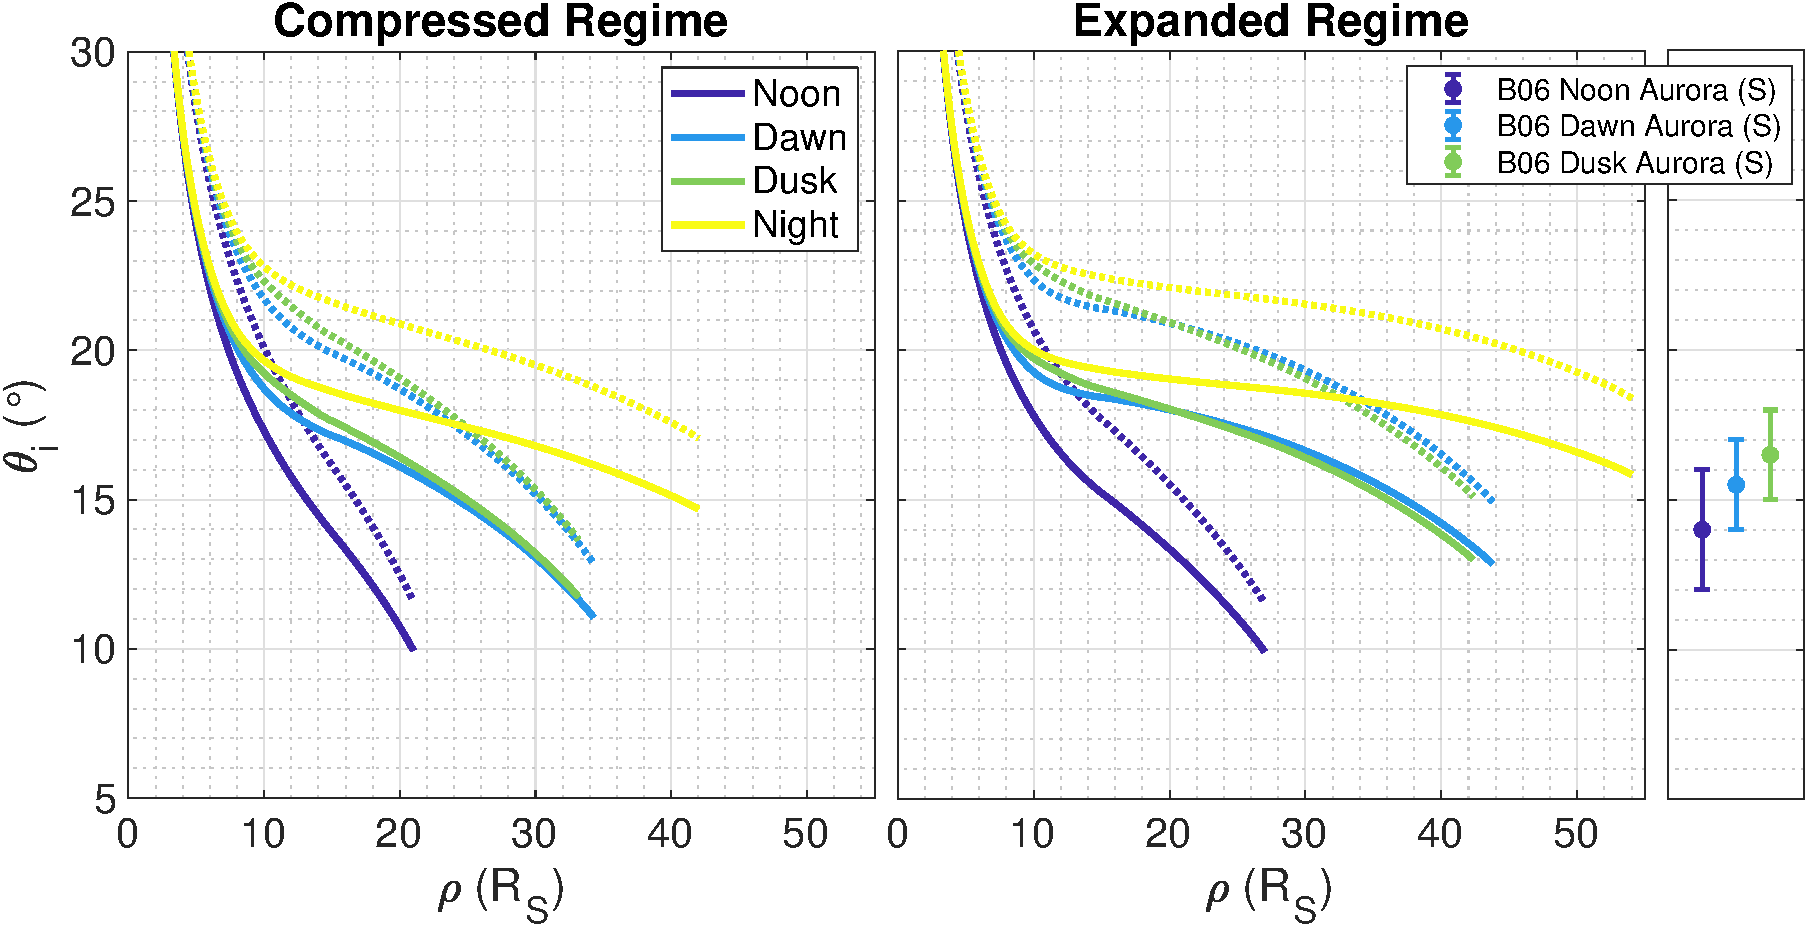
\includegraphics[width=0.9\textwidth]{LTsectors/fieldlinemapping.pdf}
\caption[Model equatorial profiles of field line mappings from the equator to the ionosphere, for different local time sectors, for the compressed and expanded regimes.]{Equatorial profiles showing the mapping of magnetic field lines from the equatorial plane to the northern (solid lines) and southern (dotted lines) ionosphere, with local time sector shown by the colour in the legend. Ionospheric colatitude $\theta_\mathrm{i}$ is measured relative to the northern pole for northern hemisphere values, and the southern pole for southern hemisphere values. Also shown by the solid circles with error bars are median locations and widths of the main auroral oval in the southern hemisphere for different local time sectors as shown by the colour, from a statistical study by \citet{badman2006}.}
\label{LTsectors:fig:fieldlinemapping}
\end{figure}

The resulting values are shown in Figure~\ref{LTsectors:fig:fieldlinemapping}, with northern hemisphere values shown by solid lines and southern hemisphere counterparts shown by dotted lines. Also shown by the coloured solid circles with error bars are the median locations and widths of the main auroral oval for noon, dawn and dusk local time sectors respectively, estimated from a statistical study of multiple Hubble Space Telescope (HST) observations of the UV aurora in the southern hemisphere from \citet{badman2006}. As these observations were of the southern hemisphere only, they should be compared with the dotted lines of the model outputs.

It can clearly be seen that there is significant variation in ionospheric mapping of field lines for different local time sectors. In particular, the location of the open-closed field line boundary (OCFLB), shown by the colatitude of the most radially distant point for each profile, varies greatly between sectors. We can see that the OCFLB maps to more polar regions in the noon sector, with ${\sim}\SI{10}{\degree}$($\SI{11.5}{\degree}$) for the northern (southern) hemisphere, than for the night sector, with ${\sim}\SI{15.5}{\degree}$($\SI{17.5}{\degree}$) for the northern (southern) hemisphere. This behaviour is qualitatively in agreement with the results of \citet{carbary2018}, who find corresponding values of ${\sim}\SI{13}{\degree}$($\SI{16}{\degree}$) for the dayside, and ${\sim}\SI{16}{\degree}$($\SI{18}{\degree}$) for the nightside, using a data-based magnetic field model. Our noon sector values are somewhat lower than the dayside values of \citet{carbary2018}; however, if we were to consider some combination of our noon, dawn and dusk values to represent the entire dayside hemisphere, for a more appropriate comparison, they would likely be in better agreement. This is because the values of OCFLB colatitude for dawn and dusk are both higher than the noon value alone.

In addition, for the compressed regime in particular, we find a slight dawn-dusk asymmetry in the location of the OCFLB, with the dusk location around $\SI{1}{\degree}$ equatorward of the dawn location. It can be seen on close inspection of Figure~\ref{LTsectors:fig:fieldlinemapping} that this asymmetry is mainly due to the small asymmetry in magnetopause radius in these models, rather than the influence of the hot plasma pressure profiles on the magnetic field structure. This is evident as the two profiles are broadly coincident in the outer magnetosphere until the dusk model terminates at $\rho=\SI{33.2}{R_S}$, in comparison to dawn's $\SI{34.3}{R_S}$. It is interesting to note that this relationship is qualitatively similar to that observed by \citet{badman2006}, who found that on average the main auroral oval in the dusk sector was located ${\sim}\SI{1}{\degree}$ equatorward of the aurora in the dawn sector, in the southern hemisphere. Furthermore, the dawn aurora was observed to be ${\sim}\SI{1.5}{\degree}$ equatorward of the noon auroral location in \citet{badman2006}. This is approximately the same as the difference in the OCFLB we observe between our noon and dawn models for the compressed regime, southern hemisphere values, as shown in the first panel of Figure~\ref{LTsectors:fig:fieldlinemapping} (although the difference is significantly higher for the expanded regime). Such a comparison supports the hypothesis from this and other studies, that the main auroral oval may map to regions in the outer equatorial magnetosphere, within a few $\si{R_S}$ of the OCFLB. In addition, a later study by \citet{badman2011} of Saturn's infrared aurora found that the nightside main oval was persistently ${\sim}\SI{2}{\degree}$ equatorward of the dayside, in line with the aforementioned day-night asymmetry we observe in our OCFLB. It is interesting to note that this agreement is achieved despite the shielding field associated with the UCL/AGA model, discussed in Section~\ref{intro:sec:forcebalancemodel} and throughout this thesis, being a less accurate approximation in the higher latitude regions, beyond around $\SI{50}{\degree}$ latitude \citep{caudal1986}.

Now comparing the results for the compressed and expanded regimes, we see that the differences between the profiles are not as extreme as the differences between local time sectors. This suggests that variations in external solar wind conditions do not have a significant impact on the magnetic mapping between ionosphere and the equatorial disc. In particular for the noon sector, the profiles for the compressed and expanded regimes are very similar, with near coincident locations of the OCFLB, and similar regions of the equatorial magnetosphere mapping to similar values of $\theta_\mathrm{i}$ in each case. For example, the equatorial radial distance corresponding to the outer one-third of the noon sector magnetosphere for each regime, maps to roughly the same $\theta_\mathrm{i}$ for each case, ${\sim}\SI{14}{\degree}$ in the north, and ${\sim}\SI{16.5}{\degree}$ in the south. A similar result was found in \citet{bunce2008}, who used an adapted ``CAN'' type \citep{connerney1981b,connerney1983} ring current model from \citet{bunce2007} to investigate how ionospheric mapping varied with system size in the noon sector magnetosphere. They found only a very modest variation with system size, for a noon magnetopause radius range of $16-\SI{26}{R_S}$, comparable to the range in this work. \citet{bunce2008b} then used the results of this modelling, in combination with HST observations of the UV aurora and \textit{Cassini} data, to show that the noon aurora are indeed likely to lie near the boundary between open and closed magnetic field lines. These authors go on to suggest that the quasi-continuous main auroral oval corresponds to the OCFLB at other local time sectors, in line with our interpretation here. Combining results for all local time sectors and compressed/expanded regimes, we find a mean location of the OCFLB equal to $\SI{12.4}{\degree}$ in the north and $\SI{14.4}{\degree}$ in the south. This is comparable to recent results from a \textit{Cassini} multi-instrument study from \citet{jinks2014}, who find corresponding values of $\SI{13.3}{\degree}$ in the north and $\SI{15.6}{\degree}$. In that study, the majority of observations are from the post-midnight sector where we expect the OCFLB to be more equatorward, which may explain why their average values are a little higher than ours.

\begin{figure}
\centering
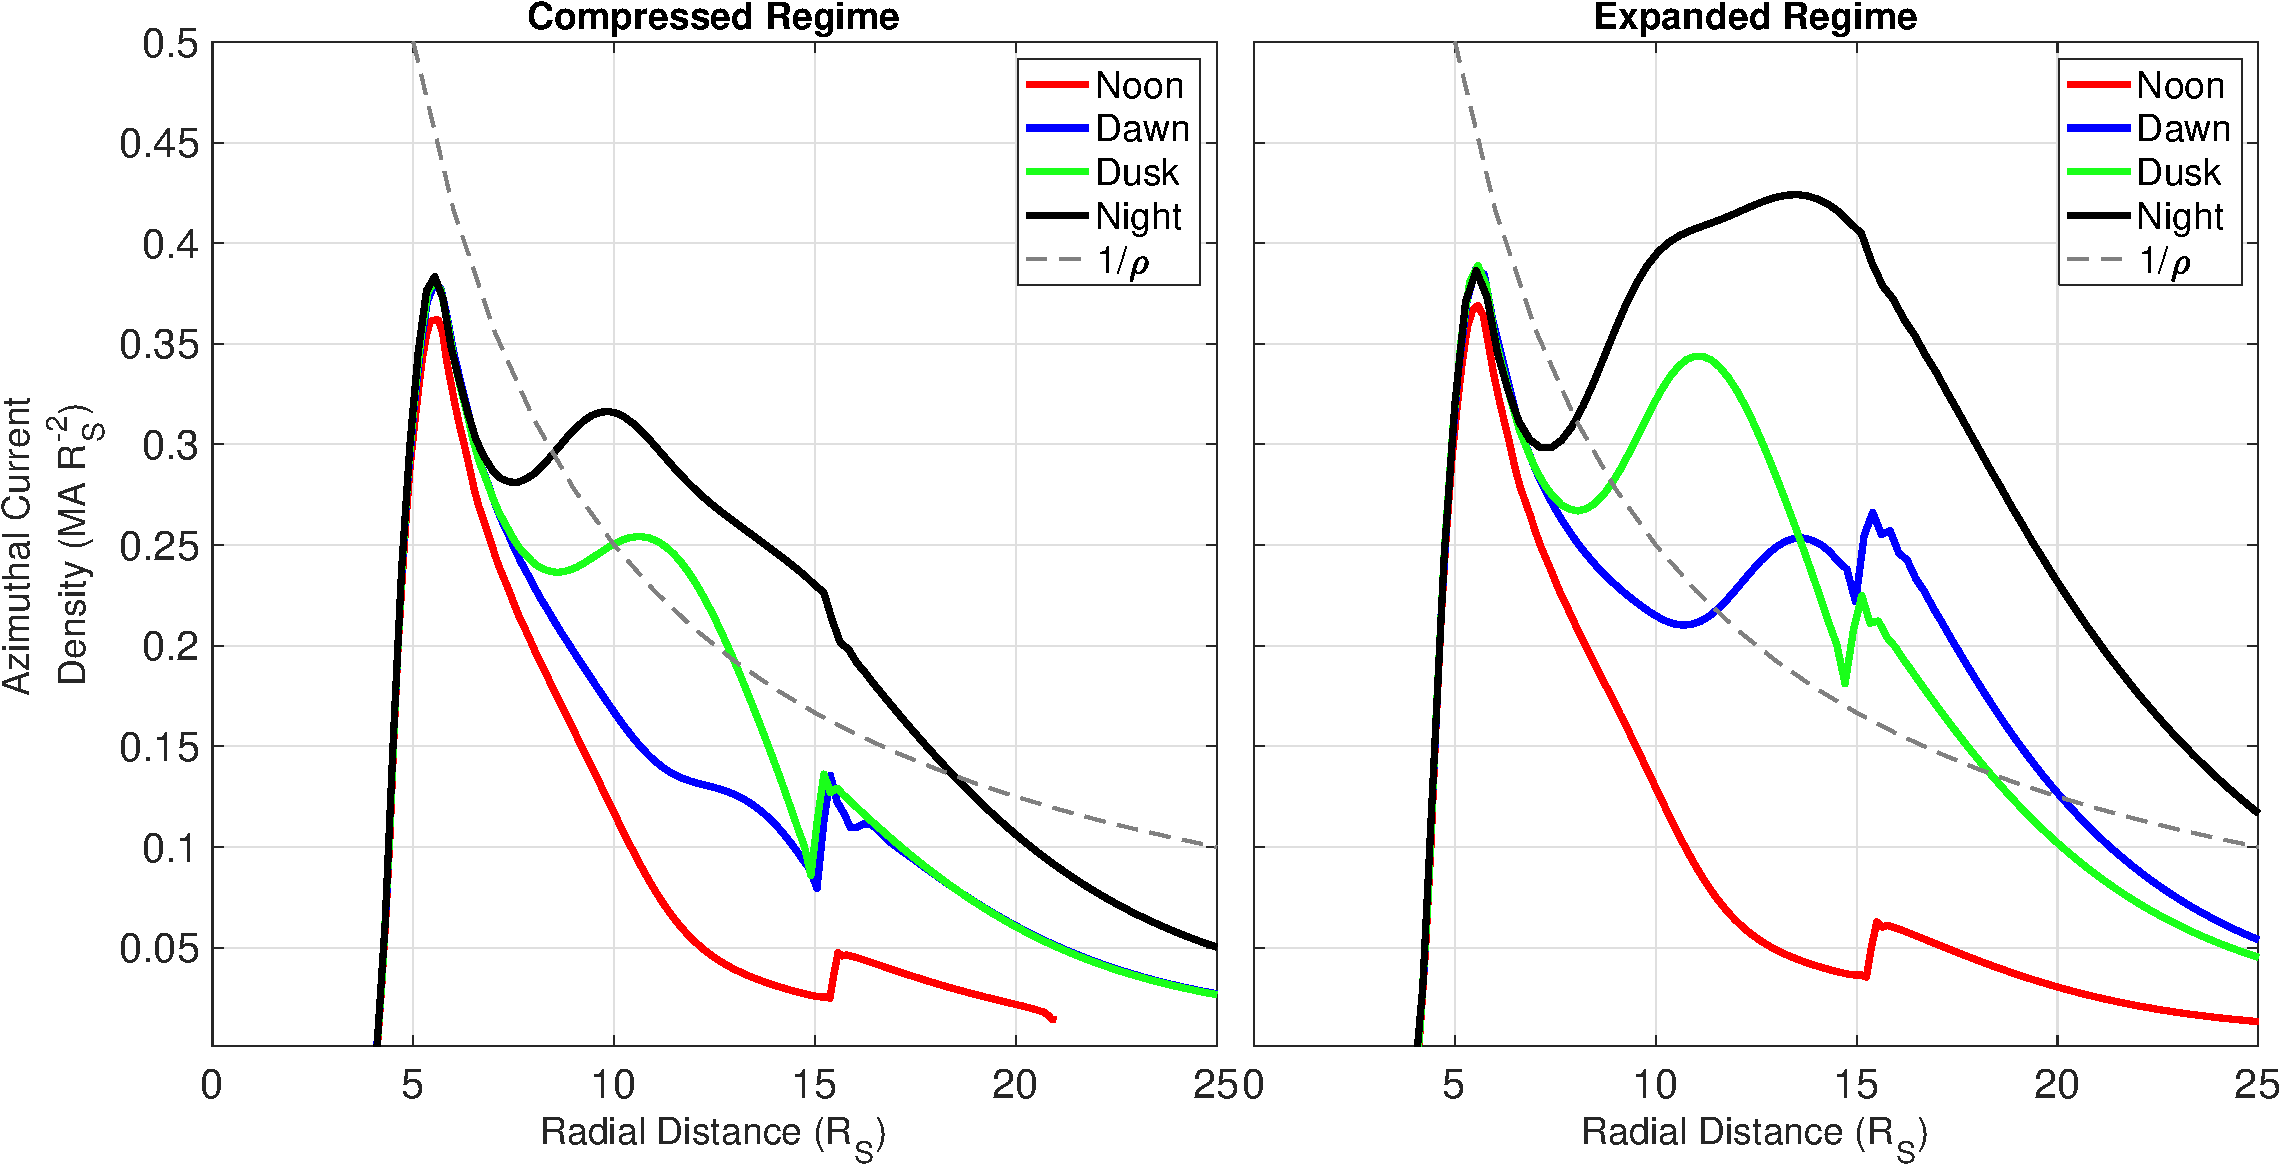
\includegraphics[width=0.8\textwidth]{LTsectors/currentdensity.pdf}
\caption[Model equatorial profiles of azimuthal current density for different local time sectors, for compressed and expanded regimes.]{Profiles of equatorial azimuthal current density with radial distance, for each local time sector model as shown by the colour, for compressed (left) and expanded (right) regimes. The grey dashed line shows a representative profile with current density inversely proportional to radial distance, as for a \citet{connerney1981b, connerney1983} style ring current model.}
\label{LTsectors:fig:currentdensity}
\end{figure}

When interpreting ionospheric-equatorial magnetic mappings, it is also pertinent to consider how the total current density varies with radial distance in the equatorial magnetosphere. Predictions for total azimuthal current density at the equator for each local time sector model, for compressed and expanded regimes, are shown in Figure~\ref{LTsectors:fig:currentdensity}. (Note that as the magnetodisc model is azimuthally axisymmetric, and hence used here to represent individual local time sectors separately, radial currents are not directly predicted.) Superimposed on each plot is a representative profile with azimuthal current density inversely proportional to cylindrical radial distance $\rho$, as is the case for CAN type ring current model constructions from \citet{connerney1981b,connerney1983}.

We can clearly see significant dawn-dusk and noon-night asymmetry in the current density profiles, with higher magnitudes for the dusk and night sector models, for both the compressed and expanded regimes. This is due to the similar relationship between the different input equatorial hot plasma pressure profiles for each local time sector, shown in Figure~\ref{LTsectors:fig:hotPpolys}, enhancing the component of the ring current associated with the hot plasma pressure gradient. In addition, the underlying magnetic field structure, and the centrifugal force on the cold plasma, both influence the current density profile via force-balance as in equation~(\ref{intro:eq:forcebalance}). This helps explain the significant difference in all profiles between the compressed and expanded regimes, with larger models having in general higher magnitude predicted azimuthal currents, due to lower magnetic field strengths at the equator as shown in Figure~\ref{LTsectors:fig:eqBfield}. The nightside models in particular have much higher predicted current densities than all other sector models for this reason. Similar results were also shown in a study by \citet{jia2012a}; in that study, the authors presented results of MHD simulations of Saturn's magnetosphere and ionosphere, and found that the predicted azimuthal current density had a persistent local time asymmetry, being higher by a factor of ${\sim}2{\--}3$ on the nightside than at other local times. In addition, it is interesting to note that for the expanded regime, the region $\rho \approx {13}{R_S}$ where the current density at dawn surpasses the current density at dusk, is almost coincident with the region where the dawn magnetic field structure becomes more disc-like than dusk, as shown in Figure~\ref{LTsectors:fig:discyness2}. This further illustrates the relationship between ring current activity and magnetodisc magnetic field structure.

From Figure~\ref{LTsectors:fig:currentdensity} we can also see that for all local time sectors, beyond the local maximum region, the equatorial current density falls more quickly than the $1/\rho$ decrease predicted by a CAN type ring current model. Similar behaviour was also found in the observational study from \citet{sergis2017}, who used \textit{Cassini} MAG, MIMI and CAPS observations to make estimates of equatorial azimuthal density profiles, and found local maxima for each sector profile in the radial range ${\sim}7{\--}\SI{13}{R_S}$, followed by a fast decay with radial distance. This suggests that the flexible ring current structure enabled by the modified UCL/AGA model used in this study may be more appropriate at characterizing the structure of Saturn's equatorial current sheet than a CAN type model. However both types of model give similar predictions for the magnetic field away from the edges of the CAN disc, as discussed in \citet{achilleos2010a}.

\section{Summary and Conclusions of this Chapter} \label{LTsectors:sec:conclusions}
In this study we have used the 2-D, force-balance UCL/AGA model from \citet{achilleos2010a} to describe the typical, equilibrium conditions of Saturn's magnetosphere at four different local time sectors. We have used equatorial profiles of hot plasma pressure at different local times from \citet{sergis2017}, and a magnetopause surface model from \citet{pilkington2015b}, to investigate how global hot plasma content and system size influence the magnetospheric structure at different local times.

We have found that, as expected, there is significant day-night asymmetry in the magnetic field structure of the magnetosphere, and that this is mainly due to the large asymmetry in magnetopause radius between day and night. We also find a small dawn-dusk asymmetry in the magnetic field structure, with both the hot plasma content and magnetopause radius having comparable influence. For the compressed regime, where the magnetosphere is under high solar wind dynamic pressure conditions, we find that the dusk sector magnetic field is more disc-like due to the influence of the increased hot plasma pressure in that sector. Meanwhile for the expanded regime we find the opposite is true, and that the dawn magnetic field is more disc-like, due to the larger magnetopause radius at dawn for this regime. Importantly, we also find significant differences in how equatorial magnetic field lines map to the polar ionosphere for the different local time sector models, with field lines from the outer magnetosphere mapping to far more equatorward regions of the ionosphere on the nightside than the dayside. This result is useful in particular when interpreting auroral observations at Saturn's ionosphere and attempting to ascertain their origins in the magnetosphere. These results may also be useful for future studies looking at local time variations in other magnetospheric properties, such as current sheet thickness.

The simplicity of the modelling approach used in this work means that many magnetospheric properties can be easily compared between different local time sectors. However a consequence of this is that any dynamical behaviour, such as reconnection events or plasmoids, cannot be directly captured. In addition, due to the assumed axisymmetry of each model, we cannot investigate the influence of any observed local time asymmetry in azimuthal phenomena. For example, a non-negligible dawn-dusk asymmetry in the azimuthal `bend-back' of magnetic field lines in the direction opposite to planetary rotation has been observed, with more substantial bend-back in the dawn sector than the dusk sector \citep[e.g.][]{delamere2015}. This may affect our assumptions of how magnetospheric plasma properties vary with radial distance, such as the angular velocity, which in turn influences our estimates of centrifugal force. In \citet{jia2016}, the authors offer a formulation for how the force balance assumption of equation~(\ref{intro:eq:forcebalance}) could be modified to account for a local time variation in radial outflow of plasma. While a preliminary investigation suggests this approach would not have a significant impact on our results, it would be worthwhile to investigate this further in a future study.

In summary, the study presented in this chapter shows that there is significant local time variation in the magnetic field structure of Saturn's magnetosphere, based on UCL/AGA model calculations. The equatorial current sheet thickness, current density and magnetic mapping to the ionosphere all vary depending on both local time and external solar wind pressure conditions, due to force balance within the magnetosphere in the UCL/AGA model. Our results are useful for potential future studies looking to interpret a range of phenomena at Saturn, from reconnection events and plasmoids to auroral oval locations and modulations. 